

\subsection{Implémentation}
\begin{frame}{Outils numériques : Feel++ }

  \begin{itemize}
  \item Méthode de Galerkin d'ordre arbitraire (cG, dG) en 1D, 2D et 3D% Supports generalized arbitrary order Galerkin methods (cG, dG) in 1D, 2D and 3D
    %\item Supporte les maillages d'ordre élevé (simplex, hypercube)
    %\item Supports generalized arbitrary order Galerkin methods (cG, dG) in 1D, 2D and 3D
    %\item Supports simplex, hypercube, high order meshes and geometries
  \item Langage très proche des mathématiques (DSEL in C++)
    %$\Longrightarrow$ DSEL  (FreeFem++)
    \begin{itemize}
    \item Expressivité : { \scriptsize modèles physiques et méthodes numériques (\alert{haut niveau})} \\
    \item Efficacité : { \scriptsize assemblages et résolutions algébriques (\alert{bas niveau})}
    \end{itemize}
  \end{itemize}


      \begin{columns}
        \column[c]{.4\textwidth}
        \scriptsize
        \vspace*{-0.07\textwidth}

        \begin{eqnarray*}
          \left\{
          \begin{aligned}
            \text{Trouver } &u \text{ qui vérifie :} \quad\quad \\
            -\Delta u &= 1 \ \ \text{dans} \ \Omega \\
            u &= 0 \ \ \text{sur} \ \partial\Omega
          \end{aligned}
          \right. \\
          \fbox{$\underset{\text{variationnelle}}{\overset{\text{Formulation}}{\Longrightarrow}}$} \quad\quad\quad\quad \\
          \left\{
          \begin{aligned}
            \text{Trouver } &u\in V_h \text{ tel que } \\
            \int_\Omega \nabla u \cdot \nabla v &= \int_\Omega v , \quad \forall v \in V_h
          \end{aligned}
          \right.
        \end{eqnarray*}

        \column[c]{.6\textwidth}

        %  \footnotesize
        \begin{block}{}
          %\begin{center}
          %\lstinputlisting[frame={top,bottom},basicstyle=\tiny]{codes/codeIntroLaplacian.cpp}
          \lstinputlisting[frame={top,bottom},basicstyle=\tiny]{codeIntroLaplacian2.cpp}
          %\end{center}
        \end{block}
      \end{columns}


\end{frame}

\begin{frame}{Pourquoi utiliser Feel++}
%\begin{block}{Pourquoi utiliser Feel++}
\begin{itemize}
\item Algèbre linéaire (structure de donnée et solveur)
\item Maillages, espaces de fonction, interpolation
\item Calcul intégrale : %TODO BC
$\int_{0}^{2\pi} \int_{0}^{\frac{\pi}{2}} Rd\frac{1}{\pi v} \vec{v}'w(\vec{r},\theta',\phi',t) sin \theta' d\theta' d\phi'$
\item Visualisation des résultats
\item Les outils de Feel++ sont paralleles
\end{itemize}
%\end{block}

\end{frame}

%%%%%%%%%%%%%%%%%%%%%%%%%%%%%%%%%%%%%%%%%%%%%%%%%%%%%%%%%%%%%%%%%%%%%%%%%%%%%%

\begin{frame}{Quelques détails d'implémentations}

%% \begin{block}{Construction de l'espaces de fonctions éléments finis et différences finis}
%% \begin{itemize}
%% \item Chargement du maillage 3d et création de l'espace élements finis
%% \item Extraction de sous maillages 1d comme base de l'espace différence fini
%% \item Correspondance des degrés de liberté entre E.F et D.F
%% \end{itemize}
%% \end{block}
%\begin{block}{Relation entre les espaces de fonctions éléments finis et différences finis}
\begin{block}{Correspondance entre les degrés de liberté éléments finis et différences finis}
  \begin{figure}[H]
    \centering
    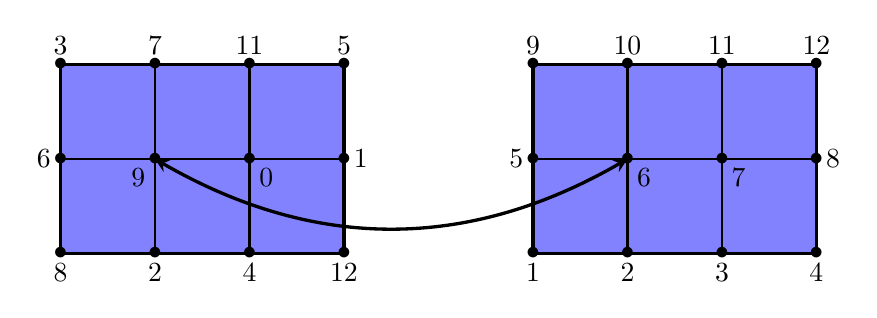
\begin{tikzpicture}[scale=1.2]

      %\draw[very thick,draw=black,fill=white!30!blue!70] (0.3,-0.15) -- (0.8,-0.15) -- (0.8,-1) -- (0.3,-1) --cycle {};
      \draw[very thick,draw=black,fill=white!30!blue!70] (0,0) -- (3,0) -- (3,2) -- (0,2) --cycle {};
      \draw[thick,draw=black] (1,0) -- (1,2);
      \draw[thick,draw=black] (2,0) -- (2,2);
      \draw[thick,draw=black] (0,1) -- (3,1);
      \draw (0,0) node {$\bullet$};
      \draw (0,0) node[below] {8};
      \draw (1,0) node {$\bullet$};
      \draw (1,0) node[below] {2};
      \draw (2,0) node {$\bullet$};
      \draw (2,0) node[below] {4};
      \draw (3,0) node {$\bullet$};
      \draw (3,0) node[below] {12};
      \draw (0,1) node {$\bullet$};
      \draw (0,1) node[left] {6};
      \draw (1,1) node {$\bullet$};
      \draw (1,1) node[below left] {9};
      \draw (2,1) node {$\bullet$};
      \draw (2,1) node[below right] {0};
      \draw (3,1) node {$\bullet$};
      \draw (3,1) node[right] {1};
      \draw (0,2) node {$\bullet$};
      \draw (0,2) node[above] {3};
      \draw (1,2) node {$\bullet$};
      \draw (1,2) node[above] {7};
      \draw (2,2) node {$\bullet$};
      \draw (2,2) node[above] {11};
      \draw (3,2) node {$\bullet$};
      \draw (3,2) node[above] {5};

    \def\shiftX{5};
      \draw[very thick,draw=black,fill=white!30!blue!70] (0+\shiftX,0) -- (3+\shiftX,0) -- (3+\shiftX,2) -- (0+\shiftX,2) --cycle {};
      \draw[thick,draw=black] (1+\shiftX,0) -- (1+\shiftX,2);
      \draw[thick,draw=black] (2+\shiftX,0) -- (2+\shiftX,2);
      \draw[thick,draw=black] (0+\shiftX,1) -- (3+\shiftX,1);
      \draw (0+\shiftX,0) node {$\bullet$};
      \draw (0+\shiftX,0) node[below] {1};
      \draw (1+\shiftX,0) node {$\bullet$};
      \draw (1+\shiftX,0) node[below] {2};
      \draw (2+\shiftX,0) node {$\bullet$};
      \draw (2+\shiftX,0) node[below] {3};
      \draw (3+\shiftX,0) node {$\bullet$};
      \draw (3+\shiftX,0) node[below] {4};
      \draw (0+\shiftX,1) node {$\bullet$};
      \draw (0+\shiftX,1) node[left] {5};
      \draw (1+\shiftX,1) node {$\bullet$};
      \draw (1+\shiftX,1) node[below right] {6};
      \draw (2+\shiftX,1) node {$\bullet$};
      \draw (2+\shiftX,1) node[below right] {7};
      \draw (3+\shiftX,1) node {$\bullet$};
      \draw (3+\shiftX,1) node[right] {8};
      \draw (0+\shiftX,2) node {$\bullet$};
      \draw (0+\shiftX,2) node[above] {9};
      \draw (1+\shiftX,2) node {$\bullet$};
      \draw (1+\shiftX,2) node[above] {10};
      \draw (2+\shiftX,2) node {$\bullet$};
      \draw (2+\shiftX,2) node[above] {11};
      \draw (3+\shiftX,2) node {$\bullet$};
      \draw (3+\shiftX,2) node[above] {12};

      \draw[<->,>=stealth,very thick] (1,1) to[bend right] (1+\shiftX,1);


    \end{tikzpicture}
  \end{figure}
\end{block}

\begin{block}{Pourquoi construire cette relation?}
  \begin{itemize}
  \item Calcul d'intégrale sur un bord ou l'ensemble du domaine
  \item Visulation de la solution différence fini
  \item projection, derivation, ... (operateurs de Feel++)
  %\item Correspondance des degrés de liberté entre E.F et D.F
  \end{itemize}
\end{block}



\end{frame}

\begin{frame}{Quelques détails d'implémentations}

\begin{block}{Discrétisation du vecteur direction}
  \begin{columns}
    \column[c]{.65\textwidth}

  \begin{itemize}
  \item Chargement d'un maillage 2d $\left[0,\pi\right] \times \left[0,2\pi\right]$  \\ ( x-coord: $\theta$, y-coord: $\phi$ )
  \item Calcul du vecteur direction à chaque noeud du maillage $\vec{v}_{ij} = F(\theta_{i},\phi_{j})$
  \end{itemize}

    \column[c]{.35\textwidth}

  \vspace*{-0.35\textwidth}
\begin{figure}[htb]
  \centering
  %,height=0.3\textheight
  \subfigure[]{
    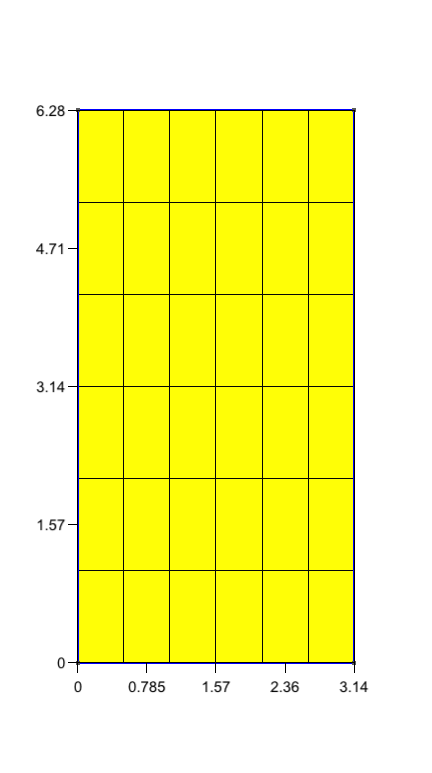
\includegraphics[width=0.4\textwidth]{Figures/acoustic-vecpropagation} 
  }
  \subfigure[]{
    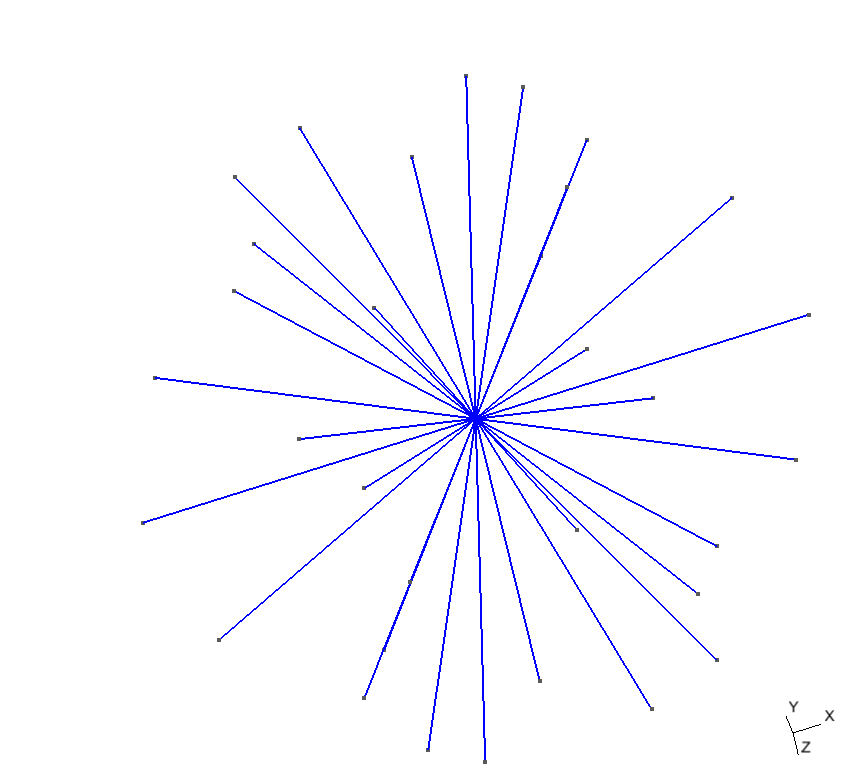
\includegraphics[width=0.4\textwidth]{Figures/allvectordirection} 
  }
\end{figure}
  \end{columns}

\end{block}

\begin{block}{Calcul de $w(\vec{r},\hat{\theta},\hat{\phi},t)$}
  \begin{itemize}
  \item Localisation du point $(\hat{\theta},\hat{\phi})=(\pi-\theta,\pi-\phi)$ dans le maillage 2d
  \item Interpolation linéaire de $w(\vec{r},\hat{\theta},\hat{\phi},t)$
  \end{itemize}
\end{block}



\end{frame}

%%%%%%%%%%%%%%%%%%%%%%%%%%%%%%%%%%%%%%%%%%%%%%%%%%%%%%%%%%%%%%%%%%%%%%%%%%%%%%


\begin{frame}{Stratégie du solveur : $Ax=F$}

\begin{itemize}
\item Méthodes de sous-espaces de Krylov :
Chercher une approximation de la solution dans un espace dont la dimension augmente à chaque étape :
%find an approximated solution in a space which the dimension increase at each step : 
\begin{equation*}
  u^{n+1} = \underbrace{u^0}_{\text{initial guess}} + \underbrace{Span\left\{ r^0,Ar^0,...,A^{n-1}r^0 \right\}}_{\text{Krylov subspace}} \quad \text{ avec } r^k=F-Ax^k
\end{equation*}
\item GMRES, CG, BICG, FGMRES, ...
\item Vitesse de convergence dépend du nombre de conditionnement de A
\item Méthodes de sous-espaces de Krylov préconditionnées :
%Transform original system into a equivalent system which have a better conditioning :
%Left preconditioning :
 $\underbrace{M_L^{-1} A}_{\tilde{A}} \ \underbrace{x}_{\tilde{x}} = \underbrace{M_L^{-1} F}_{\tilde{F}}  $
%% %\begin{itemize}
%%  Left preconditioning :
%% $\underbrace{M_L^{-1} A}_{\tilde{A}} \ \underbrace{x}_{\tilde{x}} = \underbrace{M_L^{-1} F}_{\tilde{F}}  $
%% \item Right preconditioning :
%% $ \underbrace{ A M_R^{-1}}_{\tilde{A}}  y = F $ et $x=M_R^{-1} y$

%% \item Left and right preconditioning :
%% $\underbrace{M_L^{-1} A M_R^{-1} }_{\tilde{A}}   y = \underbrace{M_L^{-1} F}_{\tilde{F}} $ et $x=M_R^{-1} y$

%% \end{itemize}

\end{itemize}

\begin{alert}{Optimisation :}
construction de la factorisation LU comme préconditionneur et réutilisation de ce préconditionneur
pour chaque direction et pour tous les pas de temps
\end{alert}



\end{frame}


%%%%%%%%%%%%%%%%%%%%%%%%%%%%%%%%%%%%%%%%%%%%%%%%%%%%%%%%%%%%%%%%%%%%%%%%%%%%%%

\begin{frame}{Applications}
\begin{itemize}
\item Equation de transport 1d, 2d et 3d : ok !
\begin{figure}[htb]
  \centering
  %,height=0.3\textheight
  \subfigure[t0]{
    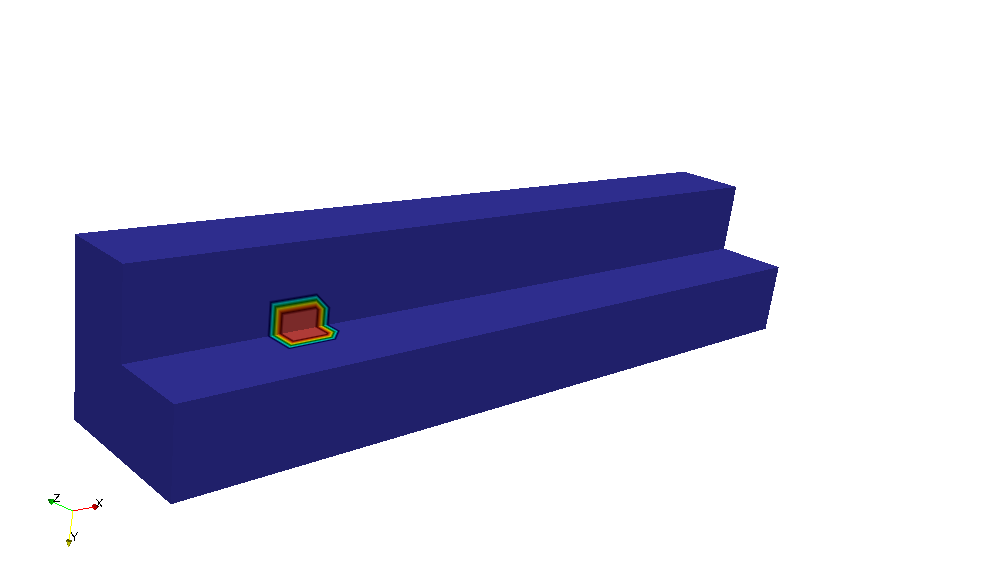
\includegraphics[width=0.25\textwidth]{Figures/simu3d_t0} 
  }
  \subfigure[t1]{
    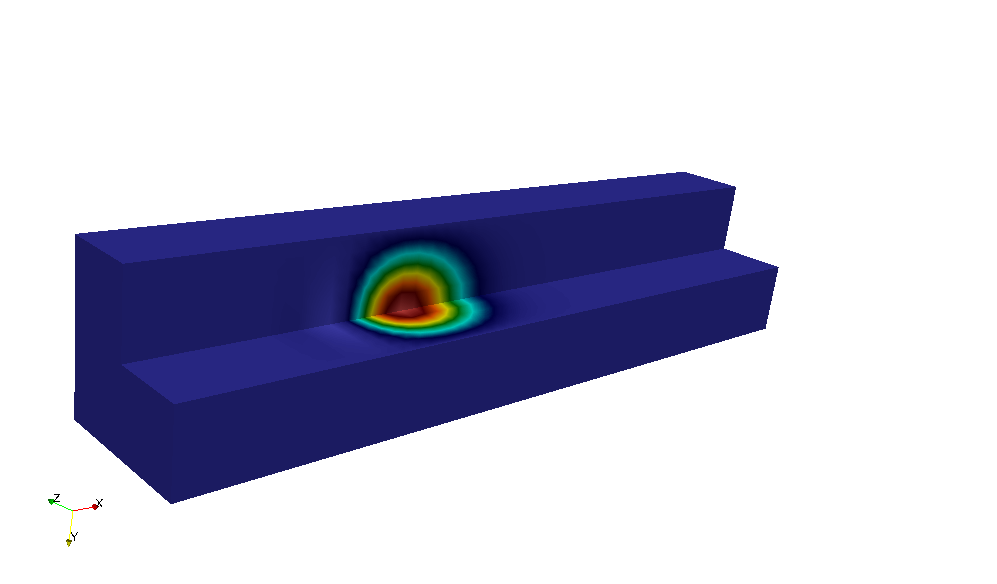
\includegraphics[width=0.25\textwidth]{Figures/simu3d_t1} 
  }
  \subfigure[t2]{
    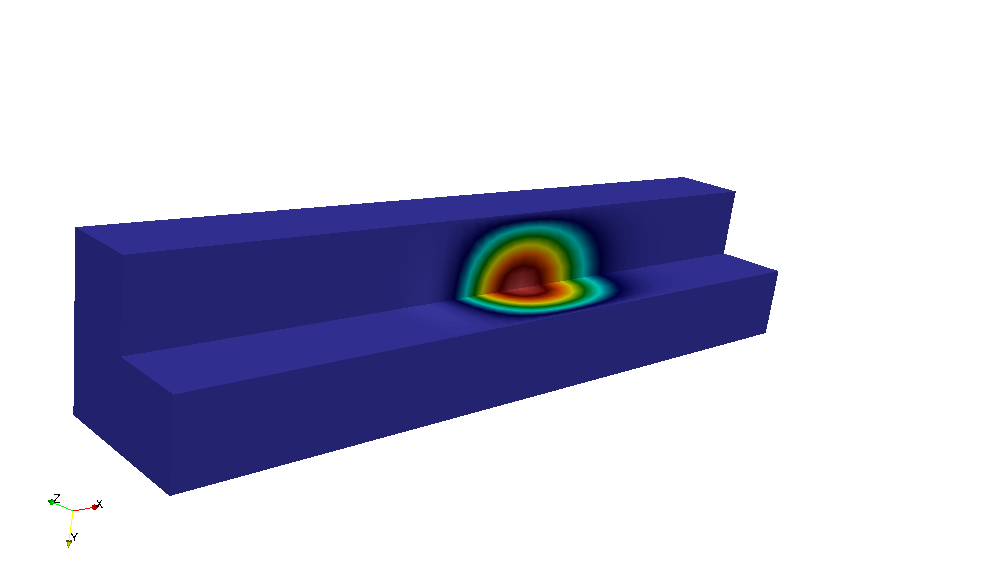
\includegraphics[width=0.25\textwidth]{Figures/simu3d_t2} 
  }
\end{figure}

\item Equation de transport 5d : {\Huge{\danger}} bug non résolu !
\end{itemize}
\end{frame}

%%%%%%%%%%%%%%%%%%%%%%%%%%%%%%%%%%%%%%%%%%%%%%%%%%%%%%%%%%%%%%%%%%%%%%%%%%%%%%
